\subsection{Neural Net Definitions}

In this document we look into a neural network based on perceptron cells with an
activation function. A single perception can be regarded as a linear classifier, i.e. it
is able to output which of two linearly separable data sets a point belongs to. In order
to classify more complex data sets, layers of perceptrons are required.

\begin{figure}[h] \centering
    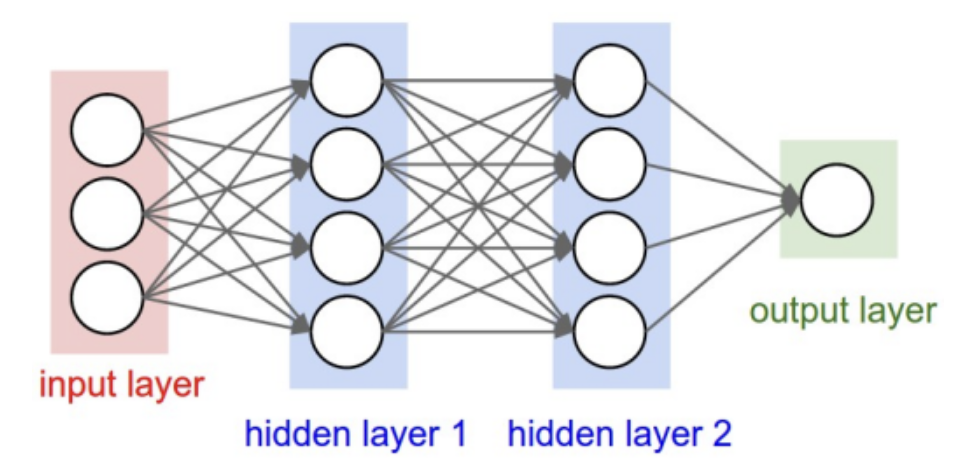
\includegraphics[width=0.75\textwidth]{neural_network} \caption{A fully
    connected Multi-Layer Perceptron (MLP) network with three inputs, two
    hidden layers, each with four perceptron nodes and an output layer with a
    single output node.} \label{fig:neural_network}
\end{figure}

A neural net consists of $L$ layers with $n^l$ nodes in each layer $l=[0,L)$. For the
input layer $(l=0)$ the nodes are simple input nodes, while for the remaining layers
consist of perceptron nodes. \\

A percptron looks like this:
\begin{figure}[h] \centering 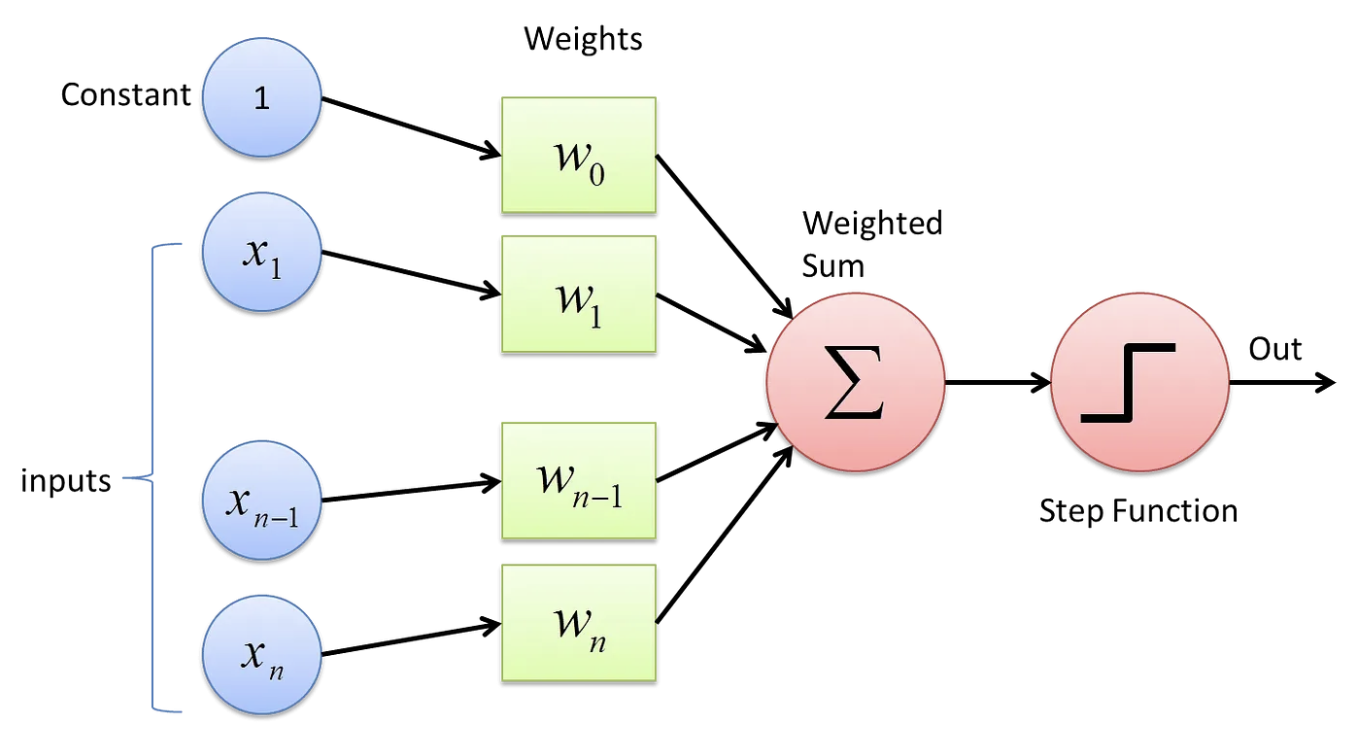
\includegraphics[width=0.75\textwidth]{perceptron_step_func}
    \caption{A Perceptron with a classical step function as activation function.}
    \label{fig:percptron_step_func}
\end{figure}

The activation function is choosen to fit the needs of the application. The nodes in the
\underline{h}idden layers $l=1$ up to $l=L-2$ have an activation function $g_h$ while the
nodes in the \underline{o}utput layer $(l=L-1)$ might have another acitivation function
$g_o$. \\

Definitions:
\begin{enumerate}
    \item (Training) \textbf{dataset} consisting of input-output pairs $(\vec{x}_i,
    \vec{y}_i)$, where $\vec{x}_i$ is the input and $\vec{y}_i$ is the desired or target
    output of the network on the input $\vec{x}_i$. The set of input-output pairs of size
    $N$ is denoted $X = \{(\vec{x}_1,\vec{y}_1), \dots, (\vec{x}_N,\vec{y}_N)\}$.
    \item A feedforward neural network whose (learning) parameters are collectivly denoted
    $\theta$. For backpropagation the parameters of primary interest are $w^l_{tf}$, the
    weight\footnote{In this notation the index $t$ stands for \emph{to}, whereas $f$
    stands for \emph{from}. Index $t$ always refers to nodes in layer $l$, while index $f$
    always refers to nodes in layer $l-1$.} between node $t$ in layer $l$ and node $f$ in
    layer $l-1$, and $b^l_t$, the bias of node $t$ in layer $l$.
    \item A loss function $L(X,\theta)$, which defines the error between the desired
    output $\vec{y}_i$ and the calculated output $\vec{o}_i$ of the neural network on the
    input $\vec{x}_i$ for a set of input pairs $(\vec{x}_i, \vec{y}_i) \in X$ and a
    particular value of the parameters $\theta$.
\end{enumerate}
The goal of training of the network is to minimize the loss function and thus to minimize
the remaining error for a given set of training data. Gradient descent is used to reduce
the error during training.\\

To define gradient descent we...

% \emph{Basis transformation:} The basis vectors of the new system expressed as a linear
% combination of the basis vectors of the old system is considered a forward transformation.
% The other direction is considered a backward transformation.\\

% Here $F$ stands for $\underline{F}$orward transformation. Basis vectors are chosen to be
% left multiplied to the transformation matrix, corresponding to summation via the first
% index of the transformation matrix. Indices are chosen upper and lower to enable the
% Einstein summation convention later on. Transformation indices are always from "north
% west" to "south east":
% \begin{equation}
%     \label{eq:forward_trafo}
%     \begin{array}{rcl}
%         [\hdbtv{1} \quad \hdbtv{2}] & = &
%         [\hdbv{1} \quad \hdbv{2}]
%         \begin{bmatrix}
%             F^{1~}_{~1} & F^{1~}_{~2} \\
%             F^{2~}_{~1} & F^{2~}_{~2}
%         \end{bmatrix} \\
%         \noalign{\vskip10pt}
%         \hdbtv{1} & = & F^{1~}_{~1}\hdbv{1} + F^{2~}_{~1}\hdbv{2}
%         \quad \underset{\text{figure}~\ref{fig:old_new_base}}{=} \quad
%         2 \hdbv{1} + 1 \hdbv{2} \\
%         \hdbtv{2} & = & F^{1~}_{~2}\hdbv{1} + F^{2~}_{~2}\hdbv{2}
%         \quad \underset{\text{figure}~\ref{fig:old_new_base}}{=} \quad
%         -\frac{1}{2}\hdbv{1} + \frac{1}{4}\hdbv{2} \\
%         \noalign{\vskip10pt}
%         \Rightarrow \hdbtvc{j} & = &
%         F^{k~}_{~j} \hdbvc{k} \quad\text{(summation convention)}
%     \end{array}
% \end{equation}

% Here $B$ stands for $\underline{B}$ackward transformation:
% \begin{equation}
%     \label{eq:backward_trafo}
%     \begin{array}{rcl}
%         [\hdbv{1} \quad \hdbv{2}] & = &
%         [\hdbtv{1} \quad \hdbtv{2}]
%         \begin{bmatrix}
%             B^{1~}_{~1} & B^{1~}_{~2} \\
%             B^{2~}_{~1} & B^{2~}_{~2}
%         \end{bmatrix} \\
%         \noalign{\vskip10pt}
%         \hdbv{1} & = & B^{1~}_{~1}\hdbtv{1} + B^{2~}_{~1}\hdbtv{2}
%         \quad \underset{\text{figure}~\ref{fig:old_new_base}}{=} \quad
%         \frac{1}{4} \hdbtv{1} + (-1) \hdbtv{2}\\
%         \hdbv{2} & = & B^{1~}_{~2}\hdbtv{1} + B^{2~}_{~2}\hdbtv{2}
%         \quad \underset{\text{figure}~\ref{fig:old_new_base}}{=} \quad
%         \frac{1}{2}\hdbtv{1} + 2 \hdbtv{2} \\
%         \noalign{\vskip10pt}
%         \Rightarrow \hdbvc{i} & = &
%         B^{j~}_{~i}\hdbtvc{j}\quad\text{(summation convention)}
%     \end{array}
% \end{equation}

% Between $B$ and $F$ following relation holds:
% \begin{equation}
%     \label{eq:forward_backward_inverse}
%     \begin{array}{rcl}
%         B^{j~}_{~i} F^{k~}_{~j} & = & F^{k~}_{~j} B^{j~}_{~i}
%         = \delta^k_i =
%         \begin{cases}
%             1, & \text{if}\ i = k \\
%             0, & \text{if}\ i \neq k
%         \end{cases} \\
%         \text{full equation transposed:} & = &
%         B^{i~}_{~j} F^{j~}_{~k} = \delta^i_k \\
%         \noalign{\vskip10pt}
%         \Rightarrow B & = & F^{-1} \quad\text{($B$ is the inverse of $F$)}
%     \end{array}
% \end{equation}


\newpage
